\chapter{DEPLOYMENT}
The process of integrating a machine learning model into an already-existing production environment is known as deployment, and it allows you to use data to make useful business choices. It can be one of the most challenging stages of the machine learning life cycle and is one of the final ones. Frequently, traditional model-building languages are incompatible with an organization's IT systems, requiring data scientists and programmers to spend considerable time and brainpower rebuilding them. A model must be successfully put into production before it can be used for making useful decisions. The effect of your model will be much diminished if you are unable to consistently derive useful insights from it.Machine learning models must be smoothly deployed into production in order for businesses to use them to start making useful judgments. This will maximize their worth.\\ 

\begin{figure}[H]
    \centering
    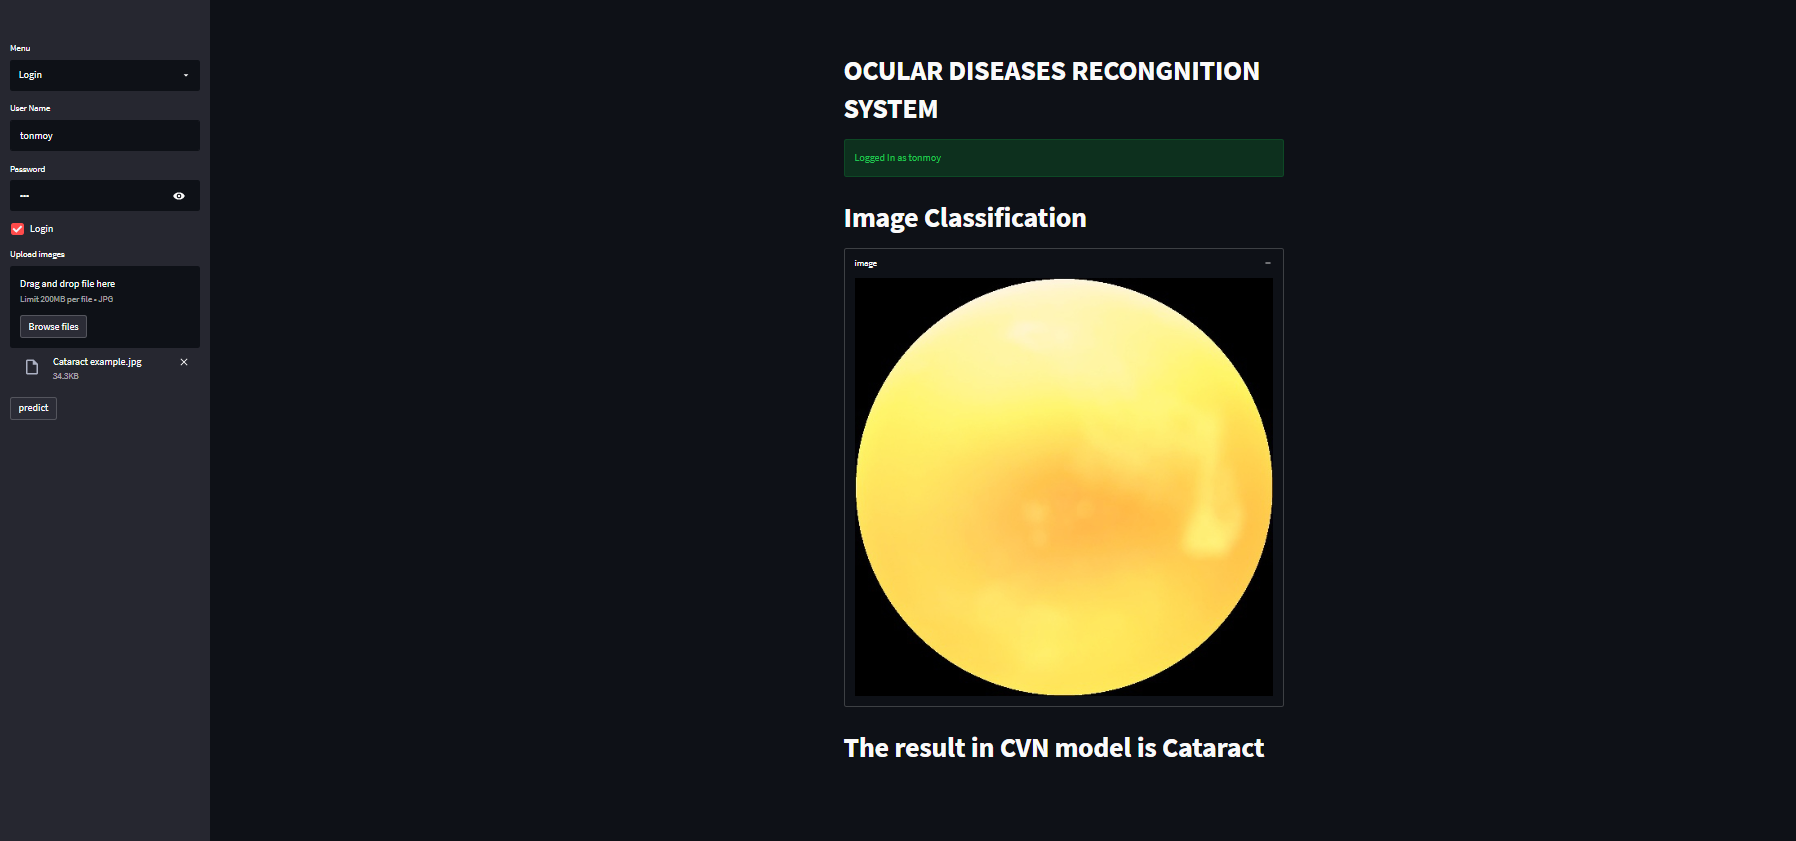
\includegraphics[scale=0.4]{70_Deployment/Deploy.png}
    \caption{Deployment}
    \label{deploy}
\end{figure}

A Python-based open source app framework is called Streamlit. It enables us to quickly develop web applications for data science and machine learning. Major Python libraries like scikit-learn, Keras, PyTorch, SymPy (latex), NumPy, pandas, and Matplotlib are all compatible with it. We used Streamlit to deploy our project.
We use Sqlite3 for temporary Data Management. Python SQLite3 module is used to integrate the SQLite database with Python. It is a standardized Python DBI API 2.0 and provides a straightforward and simple-to-use interface for interacting with SQLite databases. There is no need to install this module separately as it comes along with Python after the 2.5x version.
